\section{Friedmann Equations}
\label{sec:friedmann_eq}


%%%%%%%%%%%%%%%%%%%%%%%%%%%%%%%%%%%%%%%%%%%%%%%%%%%%%%%
%%%%% Expansion rate %%%%%
%%%%%%%%%%%%%%%%%%%%%%%%%%%%%%%%%%%%%%%%%%%%%%%%%%%%%%%
\subsection{Expansion rate}
\label{subsec:exp_rate}
According to the \emph{Cosmological Principle}, on sufficiently large scales, the universe is homogeneous and isotropic. Considering a sphere with homogeneous density and a test particle at location $\vec{x}$, and introducing a spherical coordinate system that is allowed to expand with time, due to the cosmological principle, the expansion and the time-dependent position $\vec{r}(t)$ can be expressed by
\be
\label{eq:1.5}
\vec{r} (t) = a (t) \vec{x} \,,
\ee
where $a (t)$ is the \emph{cosmic scale factor}, which does not depend only on time. For $t_0 = \mathrm{today}$, the scale factor is conventionally set to $a(t_0) = 1$. Scalar quantities $r, x$ can be used instead of $\vec{r}, \vec{x}$ due to isotropy.

The velocity of a test particle caused by cosmic expansion is
\be
\label{eq:1.6}
v(r,t) = \frac{\dd{r(t)}}{\dd{t}} = \frac{\dd{a(t)}}{\dd{t}} x = \frac{\dot{a} (t)}{a(t)} r = H(t) r \,,
\ee
which leads to the definition of the \emph{Hubble parameter}, used to quantify the relative expansion rate of the universe
\be
\label{eq:1.7}
H(t) \equiv \frac{\dot{a} (t)}{a(t)} \,,
\ee
whose value in the present epoch, $H(t_0) = H_0$, is the \emph{Hubble constant}, expressed in \cref{eq:1.3}.


%%%%%%%%%%%%%%%%%%%%%%%%%%%%%%%%%%%%%%%%%%%%%%%%%%%%%%%
%%%%% Dynamics of the expansion %%%%%
%%%%%%%%%%%%%%%%%%%%%%%%%%%%%%%%%%%%%%%%%%%%%%%%%%%%%%%
\subsection{Dynamics of the expansion}
\label{subsec:exp_dyn}
To derive the Friedmann Equations and to study the evolution of the scale factor $a (t)$, to better understand the development of the universe, one has to start from Einstein field's equation, that describes the geometry of space-time:
\be
\label{eq:1.8}
R_{\m \nu} - \frac{1}{2} R g_{\m \nu} + g_{\m \nu} \L = \frac{8 \pi G}{c^4} T_{\m \nu} \,,
\ee
where $R_{\m \nu}$ and $R$ are the Ricci tensor and Ricci scalar, respectively, $\L$ is the \emph{cosmological constant} and $T_{\m \nu}$ is the \emph{energy-momentum tensor}, which includes all contributions of energy and acts as the source of gravity.

The energy-momentum tensor of the universe is that of a homogeneous perfect fluid, characterized by its density $\r (t)$ and pressure $p (t)$. Using the Robertson-Walker metric to describe homogeneity and isotropy, the Einstein's equations simplify to the \emph{Friedmann equations} \citep{friedman_uber_1922,friedmann_uber_1924}:
\begin{subequations}
\begin{align}
    \label{eq:1.9a}
    H (t)^2 &= \bp{\frac{\dot{a}}{a}}^2 = \frac{8 \pi G}{3} \r + \frac{\L c^2}{3} - \frac{K c^2}{a^2} \,,
    \\[2ex]
    \label{eq:1.9b}
    \frac{\ddot{a}}{a} &= - \frac{4 \pi G}{3} \bp{\r + \frac{3 p}{c^2}} + \frac{\L c^2}{3} \,,
\end{align}
\end{subequations}
where $K$ is a constant parameter that defines the curvature of spatial surfaces:
\begin{itemize}
    \item $K = -1$ means open, hyperbolic space (\ie infinite) with negative curvature;
    \item $K = 0$ means flat, Euclidean space;
    \item $K = 1$ means closed, spherical space with positive curvature.
\end{itemize}

It is then possible to split up the density $\r$ into
\begin{subequations}
\begin{align}
    \label{eq:1.10a}
    \r_m (t) = \r_{m,0} a(t)^{-3} \quad &\Rightarrow \quad \textrm{non-relativistic matter} \,,
    \\
    \label{eq:1.10b}
    \r_r (t) = \r_{r,0} a(t)^{-4} \quad &\Rightarrow \quad \textrm{relativistic matter} \,.
\end{align}
\end{subequations}

Furthermore, by defining the constant vacuum energy density $\r_\L = \frac{\L}{8 \pi G}$ and the critical density $\r_{cr} = \frac{3 H_0^2}{8 \pi G}$, it is convenient to introduce dimensionless density parameters for matter, radiation and vacuum energy:
\be
\label{eq:1.11}
\O_m = \frac{\r_m}{\r_{cr}} \,, \quad\quad\quad \O_r = \frac{\r_r}{\r_{cr}} \,, \quad\quad\quad \O_\L = \frac{\r_\L}{\r_{cr}} = \frac{\L}{3 H_0^2} \,.
\ee

Finally, introducing the curvature parameter
\be
\label{eq:1.12}
\O_K = - \frac{K c^2}{H_0^2} = 1 - (\O_m + \O_r + \O_\L) \,,
\ee
and subtracting \cref{eq:1.9a} from \cref{eq:1.9b}:
\be
\label{eq:1.13}
 H (t)^2 = \bs{\frac{\dot{a}(t)}{a(t)}}^2 = H_0^2 \bs{\O_r a(t)^{-4} + \O_m a(t)^{-3} + \O_K a(t)^{-2} + \O_\L} \,.
\ee

\Cref{eq:1.13} is a fundamental equation that completely describes the expansion of the universe and contains all the information about geometry, matter, and energy content.

\begin{figure}
    \centering
    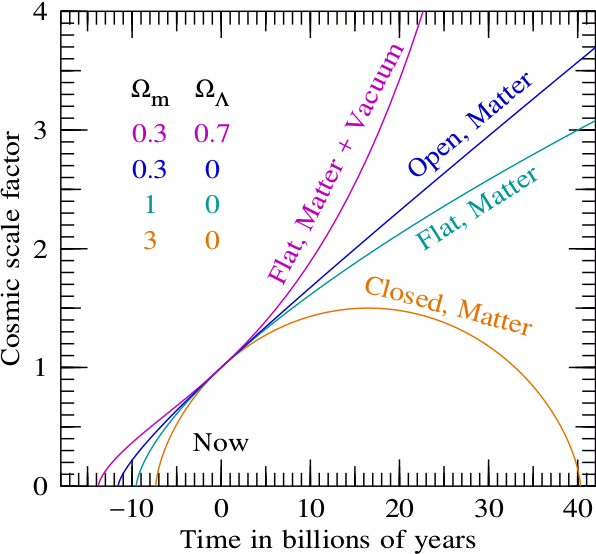
\includegraphics[width=0.65\linewidth, keepaspectratio]{img//chapter1/scalefactort.png}
    \caption[Temporal evolution of the cosmic scale factor]{Numerical solutions for \cref{eq:1.13} for different cosmological models.\\\small{Credits: \cite{hamilton_lecture_2019}.}}
    \label{fig:scalefactor}
\end{figure}


%%%%%%%%%%%%%%%%%%%%%%%%%%%%%%%%%%%%%%%%%%%%%%%%%%%%%%%
%%%%% Cosmological distances %%%%%
%%%%%%%%%%%%%%%%%%%%%%%%%%%%%%%%%%%%%%%%%%%%%%%%%%%%%%%
\subsection{Cosmological distances}
\label{subsec:dist}
In a curved space-time, there are various ways to define the distance between two points. Setting $P_0$ as the origin of a set of polar coordinates $(r, \t, \f)$ and assuming $\dd{t} = \dd{\f} = \dd{\t} = 0$, integrating the Friedmann-Robertson-Walker metric
\be
\label{eq:1.14}
\dd{s}^2 = c^2 \dd{t}^2 - a(t)^2 \bs{\frac{\dd{r}^2}{1 - K r^2} + r^2 ( \dd{\t}^2 + \sin^2{\t} \dd{\f}^2)} \,,
\ee
in this coordinate system, it is possible to determine the distance measured by a ``chain'' of observers in every point between $P_0$ and a generic point $P$ at time $t$. This is the so-called \emph{proper distance}:
\be
\label{eq:1.15}
d_P = \int_0^r \frac{a(t) \dd{r^\prime}}{\sqrt{1 - K {r^\prime}^2}} = a(t) F(r) \,,
\ee
with
\be
\label{eq:1.16}
F(r) = 
\begin{cases} 
\arcsinh(r) & \text{if } K = -1 \,;
\\
r & \text{if } K = 0 \,;
\\
\arcsin(r) & \text{if } K = 1 \,.
\end{cases}
\ee

By computing the proper distance at present time, $t = t_0$, it is possible to obtain the \emph{comoving distance}:
\be
\label{eq:1.17}
d_C \equiv d_P (t_0) = a(t_0) F (r) \,,
\ee
and since the proper distance of a source can change in time as a consequence of the time dependence of the scale factor, the source at $P$ has a radial velocity with respect to $P_0$:
\be
\label{eq:1.18}
v_r = \dot{a}(t) F(r) = \frac{\dot{a}(t)}{a(t)} d_P = H(t) d_P \,,
\ee
which is the Hubble Law mentioned in \cref{sec:history}.

There is no unique way to define the distance of an astronomical object in cosmology, and, in addition to the proper and comoving distances, which are not directly measurable, other kinds of distance can be defined that are, in principle, measurable.

Firstly, one can define the \emph{luminosity distance} of a source at a distance $r$, at time $t$ with emitted power $L$ and flux $f$:
\be
\label{eq:1.19}
d_L \equiv \sqrt{\frac{L}{4 \pi f}} \,.
\ee

Due to the expansion of the Universe it is necessary to take into account time-dilation effect, a stretch of the spherical surface centered on the source, and a cosmological redshift on the photons:
\be
\label{eq:1.20}
d_L = a(t_0) r (1 + z) \,.
\ee

Finally, the \emph{angular diameter distance}, very useful for gravitational lensing purposes, is defined as the ratio of the physical diameter $d_P$ of a source and the angle $\D \t$ that it subtends:
\be
\label{eq:1.21}
d_A = \frac{d_P}{\D \t} = a(t) r \,,
\ee
and consequently
\be
\label{eq:1.22}
d_A = d_L \frac{a(t)^2}{a(t_0)^2} = \frac{d_L}{(1 + z)^2} \,,
\ee
given that $1 + z = \frac{a(t_0)}{a(t)}$.
